\documentclass{article}

\usepackage[dutch]{babel}
\usepackage{epsfig}
\usepackage{verbatim}

\author{Peter van Dijk \& Elizabeth Schermerhorn}
\date{\today}
\title{Practicum 2 Betrouwbare communicatie}
\begin{document}
\maketitle
\newpage
\tableofcontents
\clearpage
\section{Packet Error Rate-metingen}
\subsection{Inleiding}
De Nordic RF24 is een radiozender en -ontvanger voor de 2.4GHz band. De RF24 heeft echter een aantal verschillende instellingen voor de kanalen, outputpower en datasnelheid. Het doel van dit onderzoek is bepalen wat de optimale instellingen zijn om de Packet Error Rate (PER) zo laag mogelijk te krijgen. Eerst zal de probleemstelling besproken worden samen met vastgestelde hypothesen, vervolgens zal de methodologie aan bod komen en als laatste zullen de resultaten besproken en geanalyseerd worden. 

\subsection{Probleemstelling}
De onderzoeksvraag die hier beantwoord zal worden is: \textit{"Voor welke waarden voor de outputpower, transmissiesnelheid en frequentiekanaal is de PER het laagst."} Hierbij horen de volgende hypothesen: 
\begin{enumerate}
  \item Op het moment dat er meerdere mensen op hetzelfde frequentiekanaal zitten zal dit voor veel pakket verlies zorgen.
  \item Bij een hogere outputpower zal het pakketverlies kleiner zijn.
  \item Bij een hogere transmissiesnelheid zal er meer pakketverlies optreden. 
\end{enumerate}
In het volgende onderzoek zullen deze hypothesen getoetst worden.
\subsection{Methodologie}
Om deze hypothesen te toetsen moeten er metingen gedaan worden. Hier zijn verschillende zaken van belang. 
\begin{itemize}
	\item De gebruikte hardware
	\item De gebruikte software
	\item De instellingen/vastgestelde constanten
	\item De onderzoeksopstelling
\end{itemize}

%De gebruikte hardware
\subsubsection{De hardware}
De Hardware die gebruikt is bij de metingen is een Arduino UNO en een Nordic nRF24L01 draadloze transceiver.\\

%de gebruikte software
\subsubsection{De software}
Om de hardware te gebruiken wordt gebruik gemaakt van de opensourcesoftwarebibliotheek voor de Arduino, die te vinden is op: \begin{verbatim}http://maniacbug.github.io/RF24/ \end{verbatim} 
Met deze software kan de radio aangestuurd worden en kunnen pakketjes worden verzonden en ontvangen. De radio luistert en verstuurt pakketten over een bepaald kanaal. Het is van belang dat de radio's hetzelfde kanaal gebruiken, zodat ze met elkaar kunnen communiceren. De kanalen hebben een nummer van 0 tot en met 125.\\
\\
Om de metingen uit te voeren en onze hypotheses te testen is er gebruik gemaakt van \'{e}\'{e}n zender en \'{e}\'{e}n ontvanger. De zender gebruikt \texttt{sender.ino} en de ontvanger gebruikt \texttt{receiver.ino}. Deze programma's zijn te vinden in de appendix. De zender zend pakketjes met daarin het pakketnummer. De ontvanger begint met luisteren en onthoudt het nummer van het eerste pakketje dat hij heeft ontvangen. Vervolgens zal de ontvanger blijven luisteren totdat deze 1000 pakketten heeft ontvangen. Uit de inhoud van het laatste pakket kan worden opgemaakt hoeveel pakketten er verloren zijn gegaan voor de duizend die er ontvangen zijn. De PER wordt berekend met de formule:\\
\\
\indent	(([laatste pakketnummer]-[eerste pakketnummer])/[aantal ontvangen pakketten])\\
\\
In de software van de Sender en Receiver is gebruik gemaakt van de volgende drie methoden om de verschillende waarden aan te kunnen passen. 
\begin{itemize}
	\item setChannel(uint\char`_8 i) \\
	met 0 $\leq$ i $\leq$ 125
	\item setPALevel(PALevel level) \\
	met level $\in \{$  RF24\_PA\_MAX, RF24\_PA\_MIN, RF24\_PA\_LOW $\}$
	\item setDataRate(Rate rate) \\
	met rate $\in \{$ RF24\_1MBPS, RF24\_2MBPS$\}$
\end{itemize}
Door met deze drie methoden de waarden aan te passen verkrijgen we de gewilde meetresultaten. Deze zullen in sectie 1.4 besproken worden.

\subsubsection{De instellingen/vastgestelde constanten}
Om deze metingen bruikbaar te houden moeten er een paar constanten gedefinieerd worden.
\begin{itemize}
	\item De grootte van de payload
	\item Het aantal te versturen berichten
\end{itemize}
Het aantal keer dat er een pakket opnieuw verstuurd wordt is niet van belang in deze implementatie omdat het zo ge\"{i}mplementeerd is dat het aantal ontvangen berichten wordt bijgehouden en het aantal verzonden berichten wordt bijgehouden. 
Voor de grootte van de payload is er gekozen voor de grootst mogelijke waarde die deze kan aannemen, namelijk 255 bytes. Deze waarde is gekozen omdat de onderzoeksvraag is wanneer is de radio communicatie het meest betrouwbaar en dit moet getest worden voor re\"{e}le waarden. 
Het aantal te versturen berichten is op 1000 gezet. Hier is voor gekozen vanwege het idee omdat meer waarden betekent nauwkeurigere resultaten.
\\
\\
De meetopstelling bestaat uit twee radio's welke 270cm uit elkaar geplaatst zijn. Om de resultaten consistent te houden moet bij elke meting deze afstand aangehouden worden. 
Verder worden bericht niet opnieuw verzonden als er geen acknowledgement volgt, want dit betekent pakket verlies en dat moet gemeten worden. 

\subsection{Resultaten en analyse}
Hier zullen de resultaten weergegeven en geanalyseerd worden. \\*
  De constanten zoals ze standaard gebruikt zullen worden. Als ze gewijzigd worden voor de test dan wordt dit aangegeven. 
  \begin{itemize}
  	\item afstand tussen radio's: 270 cm
  	\item Geen hertransmissie van pakketten
  	\item payload: 255 bytes
  	\item channel: 125
  \end{itemize}
  
\subsubsection{Metingen en resultaten}
Tijdens de metingen waren er geen andere radio's aan het sturen, waardoor de radio's geen last van interferentie hadden.\\
\\
    \begin{tabular}{ | l | l | l | p{5cm} |}
    \hline
    Instellingen 				& PER 		& gemiddelde PER\\ \hline
    outputpower: MAX 			& 1/1000 	& 2/3000		\\
    transmissiesnelheid: 2MBps 	& 1/1000 	& 				\\
    delay: 25 ms 				& 0/1000	&  				\\ \hline
    \end{tabular}\\
\\
\\
    \begin{tabular}{ | l | l | l | p{5cm} |}
    \hline
    Instellingen				& PER 		& gemiddelde PER\\ \hline
    outputpower: MAX 			& 0/1000 	& 0/3000		\\
    transmissiesnelheid: 2MBps 	& 0/1000 	&  				\\
    delay: 50 ms 				& 0/1000	&  				\\ \hline
    \end{tabular}\\
\\
\\
    \begin{tabular}{ | l | l | l | p{5cm} |}
    \hline
    Instellingen 				& PER 		& gemiddelde PER\\ \hline
    outputpower: MAX 			& 0/1000 	& 0/3000		\\
    transmissiesnelheid: 1MBps 	& 0/1000 	&  				\\
    delay: 50 ms 				& 0/1000	&  				\\ \hline
    \end{tabular}\\
\\
\\
    \begin{tabular}{ | l | l | l | p{5cm} |}
    \hline
    Instellingen				& PER 		& gemiddelde PER\\ \hline
    outputpower: MIN 			& 85/1000 	& 1273/3000		\\ 
    transmissiesnelheid: 2MBps 	& 669/1000  &  				\\ 
    delay: 50 ms 				& 519/1000 	&  				\\ \hline
    \end{tabular}\\
\\
\\
    \begin{tabular}{ | l | l | l | p{5cm} |}
    \hline
    Instellingen				& PER 		& gemiddelde PER\\ \hline
    outputpower: LOW 			& 0/1000 	& 8/3000		\\ 
    transmissiesnelheid: 2MBps 	& 2/1000 	&   			\\ 
    delay: 50 ms 				& 6/1000 	&  				\\ \hline
    \end{tabular}\\
\\
\\
    \begin{tabular}{ | l | l | l | p{5cm} |}
    \hline
    Instellingen				& PER 		& gemiddelde PER\\ \hline
    outputpower: MAX 			& 0/1000 	&  0/3000		\\ 
    transmissiesnelheid: 2MBps 	& 0/1000 	&   			\\ 
    delay: 50 ms 				& 0/1000 	&				\\ 
    channel: 0 					&  			&  				\\ \hline
    \end{tabular}\\
\\
\\
    \begin{tabular}{ | l | l | l | p{5cm} |}
    \hline
    Instellingen				& PER 		& gemiddelde PER\\ \hline
    outputpower: MAX 			& 0/1000 	& 1/3000		\\ 
    transmissiesnelheid: 2MBps 	& 1/1000 	&  				\\ 
    delay: 50 ms 				& 0/1000 	&  				\\ 
    channel: 64 				&  			&				\\ \hline
    \end{tabular}\\
\\
\\
Verder zijn er nog enkele kleinere tests uitgevoerd op een netwerk met interferentie. Dit leverde de volgende resultaten:\\
\\
\begin{tabular}{ | l | l | l | p{5cm} |}
    \hline
    Instellingen				& PER 		& gemiddelde PER\\ \hline
    outputpower: MAX 			& 47/300 	& 433/3000		\\ 
    transmissiesnelheid: 2MBps 	& 77/300 	&  				\\ 
    delay: 50 ms 				& 9/300 	&  				\\ \hline
    \end{tabular}\\
\\
\\
Om het resultaat nauwkeuriger en accurater te kunnen weergeven is ervoor gekozen om alle tests in drievoud uit te voeren zodat vreemde gebeurtenissen opgemerkt worden. Een voorbeeld is een error rate $>$ 1. Tussen deze resultaten is de instelling HIGH voor outputpower niet weergegeven, aangezien deze voor de gebruikte versie van de radio niet een mogelijke waarde was.

\subsection{Conclusie}
Als er naar de gevonden waarden gekeken wordt, is de PER onacceptabel wanneer de outputpower op MIN staat. Een gemiddelde PER van 1273/3000 pakketten zorgt op den duur voor veel hertransmissies dus veel vertraging op het netwerk. Dit is een situatie die niet gewenst is. Wanneer naar de overige instellingen gekeken wordt en de daarbij behorende gemiddelde PER dan zijn ze perfect of een PER $<$ 0.01. Hier moet bij vermeld worden dat op het moment dat er meer interferentie is op het netwerk de PER omhoog schiet op het netwerk. Op dat moment is het kiezen van een ongebruikt frequentiekanaal van belang. Dit experiment heeft plaats gevonden in een interferentievrije ruimte.\\
\\
De onderzoeksvraag is: \textit{"Voor welke waarden voor de outputpower, transmissiesnelheid en frequentiekanaal is de PER het laagst."} Het antwoord dat hierbij hoort is dat voor elke waarde van de transmissiesnelheid en het frequentiekanaal de PER niet boven de 0.01 uit komt. Dit geldt echter niet voor de outputpower; op het moment dat de outputpower op minimaal gezet wordt bedraagt de gemiddelde PER 1273/3000. Hieruit kan geconcludeerd worden dat de outputpower tenminste op laag of maximaal gezet moet worden om de PER tot een minimum te beperken. 

\newpage

\clearpage
\section{Betrouwbare end-to-end-communicatie}
\begin{figure}
\centering 
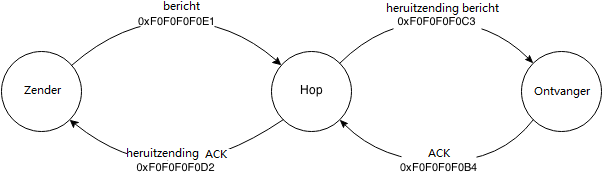
\epsfig{file=img/hop.png,width=\linewidth} 
\caption{Opstelling van het netwerk}
\label{fig:converter} %always place your label after your caption!
\end{figure}

\subsection{Inleiding}
\subsection{Probleemstelling}
\subsection{Methodologie}
\subsection{Resultaten en analyse}
\clearpage




\appendix
\section{De radio en de RF24-library}
In dit onderzoek wordt gebruik gemaakt van de rf24 radio. Deze radio heeft de volgende eigenschappen:
	\begin{itemize}	
	\item\textbf{Frequentieband: }2.4000-2.4835 GHz
	\item\textbf{Datasnelheid: }1 of 2 Mb/s
	\item\textbf{Aantal kanalen: }126 RF-kanalen
	\item\textbf{Modulatietechniek: }Gaussian Frequency Shift Key(GFSK)
	\end{itemize}
\begin{tabular}{c|c}
\textbf{Energiemodus}  & \textbf{Energieverbruik in Amp\`ere}     \\
\hline
Standby-I   & 22 $\mu$A    	\\
Standby-II  & 320 $\mu$A	\\
Power down  & 900 nA 
\end{tabular}\\
\\
\\
\begin{tabular}{c|c}
\textbf{Zendmodus}  & \textbf{Energieverbruik in Amp\`ere}     \\
\hline
0 dBm  	& 11.3 mA	\\
-6 dBm 	& 9 mA    	\\
-12 dBm & 7.5 mA  	\\
-8 dBm 	& 7 mA
\end{tabular}\\
\\
\\
\begin{tabular}{c|c}
\textbf{Ontvangstmodus}  & \textbf{Energieverbruik in Amp\`ere}     \\
\hline
2 Mbps  & 12.3 mA    \\
1Mbps	& 11.8 mA     
\end{tabular}


\section{Code Sender}
\verbatiminput{./Sender/Sender.ino}

\section{Code Receiver}
\verbatiminput{./receiver/receiver.ino}


\end{document}